\chapter{Seguridad y fiabilidad de los datos}

La seguridad de los datos se centra sobre todo en la autorización de los usuarios, es decir, cómo entrar al SGBD (autorización de usuarios). Una vez dentro, podrás hacer unas cosas u otras con esos datos (gestión de privilegios y roles).

La seguridad es necesaria ya que el SGBD debe garantizar dos cosas siempre:
\begin{itemize}
\item La exclusividad en el acceso a la información a quien tiene permisos.
\item Que se pueda recuperar cuando ocurre un fallo.
\end{itemize}

Para poder garantizar que no se dan accesos indebidos, existen varios niveles donde se puede actuar:
\begin{itemize}
\item Nivel físico: acceso a ubicación. Por ejemplo, guardar el servidor en una habitación segura.
\item Nivel humano: confianza en usuarios con permisos.
\item Nivel del S.O.: si permite conexión remota y proporciona acceso local desde conexión remota.
\item Nivel de SGBD: a nivel de información (quién accede a qué) y de operación  (qué puede hacer).
\end{itemize}

Cuando la información es sensible, siempre se recomienda cifrar los datos y las conexiones. Esto se puede hacer a nivel del sistema de ficheros, a nivel del sistema operativo a nivel del SGBD. Aunque es más seguro, esto ralentiza las operaciones porque hay que descifrar y cifrar los bloques cada vez que se usan. 

\section{Autorización de usuarios}

Normalmente en los SGBD, la autorización de usuarios presenta dos niveles de autorización: el primero es el uso de un par usuario/contraseña: cuando se crea un usuario en la BD hay que especificar su contraseña. 

El segundo trata sobre cómo y quién crea estos usuarios. Para obtener un usuario en un SGBD hay dos formas de proceder:
\begin{itemize}
\item En sistemas centralizados, el administrador lo crea todo y concede permisos.
\item En sistemas descentralizados, hay una jerarquía de usuarios con permisos que pueden concederse o cederse, según determine el propietario. Aquí también hay un usuario administrador ojo, pero delega ciertos permisos a otros usuarios.  
\end{itemize}

Este sistema de concesiones de permisos funciona usando un grafo de autorización:

\begin{figure}[H]
  \center
  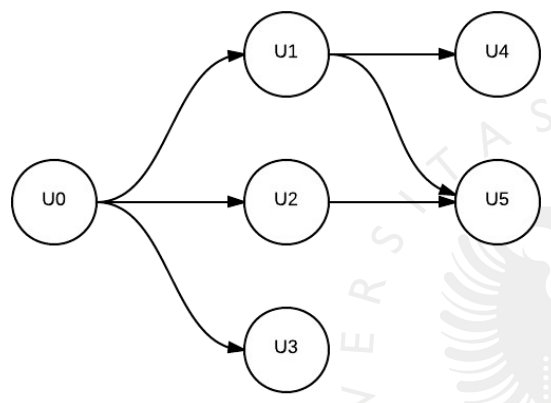
\includegraphics[scale=0.35]{img/15.png}
\end{figure}

Ojo, \textbf{ceder y conceder no es lo mismo}. Si U0 concende el permiso a U1, entonces U1 puede usarlo pero no concederlo. S U0 le cede el permiso a U2,  entonces U2 puede usar ese permiso y concederlo y cederlo a U5.

Como muestra el siguiente grafo, la cesión no es muy recomendable. Imagina que U0 le quita el permiso a U2. U2 seguiría teniendo ese privilegio ya que se lo está concediendo o cediendo U3. Por esta razón, la cesión solo se suele usar entre administradores del sistema.

\begin{figure}[H]
  \center
  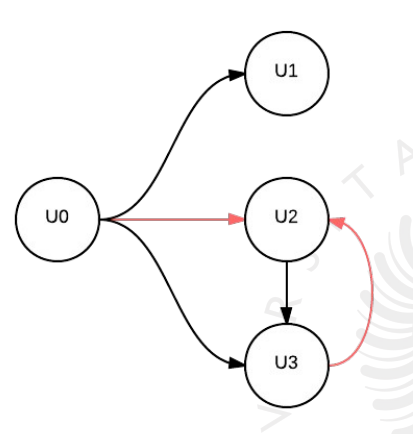
\includegraphics[scale=0.35]{img/16.png}
\end{figure}

\section{Gestión de privilegios y roles}

Un \textbf{privilegio} es un derecho a ejecutar una determinada sentencia o acceder a un determinado objeto de la base de datos. Es responsabilidad del administrador el concderle. Pueden concederse de dos formas: directamente o a través de un rol.

Un \textbf{rol} es un conjunto de privilegios con un nombre, que pueden cederse o concederse en grupo. Existen algunos roles predefinidos:
\begin{itemize}
\item CONNECT: permite conectar a la BD, consultar tablas públicas, crear vistas y exportar tablas. El usuario \textit{PUBLIC} representa a todos los usuarios con este permiso. En lugar de crear una funcionalidad nueva, se crea ese usuario y los objetos públicos los crea o se le asignan a él. Luego este rol básicamente te da acceso de lectura a todos los objetos del usuario PUBLIC.
\item RESOURCE: permite crear tablas e índices.
\item DBA: \underline{incluye a los anteriores} y permite acceder a datos de todos los usuarios, conceder y revocar privilegios, realizar mantenimiento de sistema y backups, etc. También permite exportar la BD total o parcialmente.
\end{itemize}

Existen dos tipos de privilegios dependiendo de qué es lo que permiten hacer:

\begin{itemize}
\item Privilegios de sistema: derecho a realizar una acción genérica sobre el sistema (creación de objetos, operaciones de la BD en conjunto, etc). Es decir, te permite hacer algo sobre la totalidad del sistema. Por ejemplo, casi todas las sentencias que contienen \textit{CREATE} y \textit{ANY}.

Puedes asignar o revocar estos privilegios con las siguientes órdenes:
\begin{lstlisting}[ language=SQL,
                    deletekeywords={IDENTITY},
                    deletekeywords={[2]INT},
                    morekeywords={clustered},
                    framesep=8pt,
                    xleftmargin=40pt,
                    framexleftmargin=40pt,
                    frame=tb,
                    framerule=0pt ]
GRANT <priv/role> TO <user/role/PUBLIC> [WITH ADMIN OPTION];
REVOKE <priv/role> FROM <user/role/PUBLIC>;
\end{lstlisting}
Se pueden poner en forma de lista, separándolos por coma. La opción \textit{WITH ADMIN OPTION} es lo equivalente a ceder el privelegio. Sin ella, lo estaríamos concediendo. Si revocamos un privilegio que había sido cedido a un usuario, ese privilegio también será borrado para todos los usuarios que lo hayan obtenido a partir de él. 

Una de las ventajas de esta forma es que podemos asignar roles a roles, es decir, podemos construir roles de forma incremental. 

\item Privilegios de objeto: derecho a realizar una acción particular sobre un objeto concreto (insertar tuplas,  borrar tuplas, consultar tuplas, etc). Por ejemplo: ALL, DELETE, INDEX, INSERT, SELECT, UPDATE, etc.

Para asignar o revocar estos privilegios se usa:
\begin{lstlisting}[ language=SQL,
                    deletekeywords={IDENTITY},
                    deletekeywords={[2]INT},
                    morekeywords={clustered},
                    framesep=8pt,
                    xleftmargin=40pt,
                    framexleftmargin=40pt,
                    frame=tb,
                    framerule=0pt ]
GRANT <priv/role> ON <objeto> TO <user/role/PUBLIC> [WITH ADMIN OPTION];
REVOKE <priv/role> ON <objeto> FROM <user/role/PUBLIC>;
\end{lstlisting}
\end{itemize}

Toda la información sobre privilegios y roles se pueden consultar a través de las siguientes vistas:

\begin{figure}[H]
  \center
  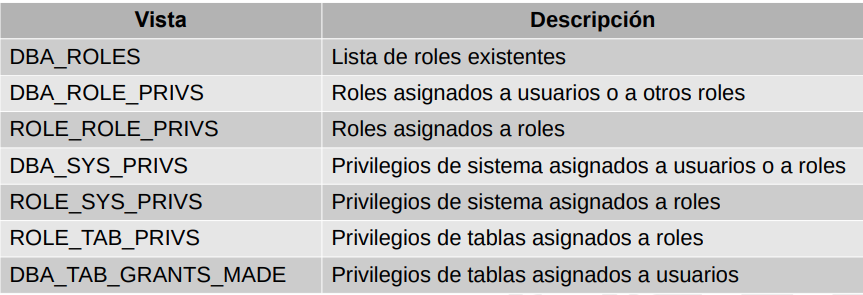
\includegraphics[scale=0.45]{img/17.png}
\end{figure}

\section{Fiabilidad de los datos}

En el SGBD se pueden dar varios errores:

\begin{itemize}
\item Errores lógicos: por problema interno (overflow, entrada inválida, etc.).
\item Errores del sistema: acceso concurrente o exceso de procesos. La transacción se ejecuta cuando se recupere el sistema.
\item Caída: fallo hardware o eléctrico.
\item Falo en almacenamiento externo: sólo salvable si tenemos copias de seguridad.
\end{itemize}

Algunas formas de sobrellevar estos fallos y asegurar la fiabilidad del sistema son:

\subsection{Transacciones}

Una transacción es una unidad lógica de procesamiento constituida por varias sentencias que deben ejecutarse en bloque o no ejecutarse.\\
Las transacciones deben verificar las propiedades ACID:
\begin{itemize}
\item Atómica (Atomicity)
\item Consistente (Consistency)
\item Aislada (Isolation)
\item Persistente (Durability)
\end{itemize}

Una transacción puede encontrarse en varios puntos. Cuando la transacción comienza, pasa al estado de \textbf{activa}. Si todas sus sentencias se han ejecutado, pero la transacción no ha finalizado todavía, entonces se encuentra \textbf{parcialmente ejecutada}. Si además termina la transacción, estará \textbf{ejecutada}. Si alguna de sus sentencias produce un fallo y la transacción no ha terminado, entonces está \textbf{parcialmente abortada}. Si además se ha terminado la transacción, entonces está \textbf{abortada}.

\begin{figure}[H]
  \center
  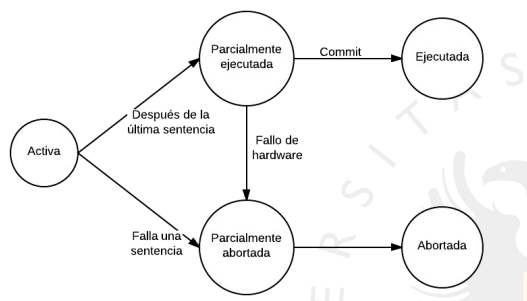
\includegraphics[scale=0.45]{img/18.png}
\end{figure}

\subsection{Gestión de bloques y buffers}

Cuando una transacción se marca como ejecutada, los bloques cambiados se encuentran en memoria y serán volcados a discos cuando sea conveniente. Por esa razón, para mantener la consistencia, necesitamos de alguna manera anotar qué se ha hecho. Las transferencias entre disco y memoria pueden tener también varios estados:

\begin{itemize}
\item Realizada con éxito (ejecutada)
\item Parcialmente fallida (parcialmente abortada)
\item Totalmente fallida (abortada)
\end{itemize}

Para manterner la consistencia, cualquier fallo tiene que ser detectado y, si ocure, el bloque destino debe quedar intacto. Una posible solución para conseguir esto es mantener dos bloques físicos por cada bloque lógico. Esto se realiza primero escribiendo uno, si no hay fallo, se escribe el otro. Será exitosa cuando se hayan realizado las dos. 

Para la recuperación: si los dos son iguales y no se detectan errores, no hay fallos. Si se produce fallo durante la lectura de uno, se copia el otro bloque encima del fallido.

\begin{itemize}
\item Operaciones entre buffers y disco:
\begin{itemize}
\item lee\_bloque(X): transfiere el bloque físico que contiene el dato X al buffer.
\item escribe\_bloque(X): transfiere el buffer que contiene el dato X al disco, reemplazando el bloque físico.
\end{itemize}
\item Operaciones entre programa y buffers:
\begin{itemize}
\item lee(X,$x_i$): lee el dato X del buffer sobre la variable local $x_i$, si es necesario, se ejecuta lee\_bloque(X).
\item escribe(X,$x_i$): asigna el valor de la variable local $x_i$ al dato X del buffer, si es necesario, se ejecuta lee\_bloque(X).
\end{itemize}
\end{itemize}

La lectura se realiza por necesidad del dato y la escritura se realiza por necesidad de espacio. 

\subsection{Tabla de modificaciones}

Si hay datos modificados en los buffers y ocurre una caída del sistema, parte de los datos pueden haber sido escritos en el disco. ¿Cómo podemos recuperar valores antiguos? Tenemos varios problemas:
\begin{itemize}
\item Determinar qué valores han sido modificados es costoso en operaciones de E/S.
\item Encontrar los valores antiguos de los datos es aún más costoso (cláusulas WHERE sobre varias tuplas).
\end{itemize}

Para evitar estos problemas lo que se hace es complicar un poco el SGBD. Los SGBD mantiene una table en memoria con las modificaciones que se quieren realizar (log) mediante inserciones, actualizaciones o borrados. A esta estructura se le denomina \textbf{tabla de modificaciones} o \textbf{bitácora}. Almacena: código de transacción, estado, operación, marca de tiempo, nombre del dato, valor antiguo y valor nuevo, aunque algunos sistemas pueden incluir más.

\begin{figure}[H]
  \center
  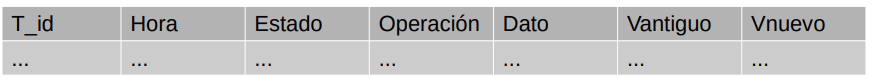
\includegraphics[scale=0.45]{img/19.png}
\end{figure}

Al comenzar una transacción, se escribe una entrada $<T_i,\text{ start }>$ con el resto de valores vacíos. Cualquier operación de una transacción, va precedida por su correspondiente entrada. Cuando termina una transacción, se escribe una entrada $<T_i, \text{ commit }>$, con el resto de valores vacíos.

\begin{figure}[H]
  \center
  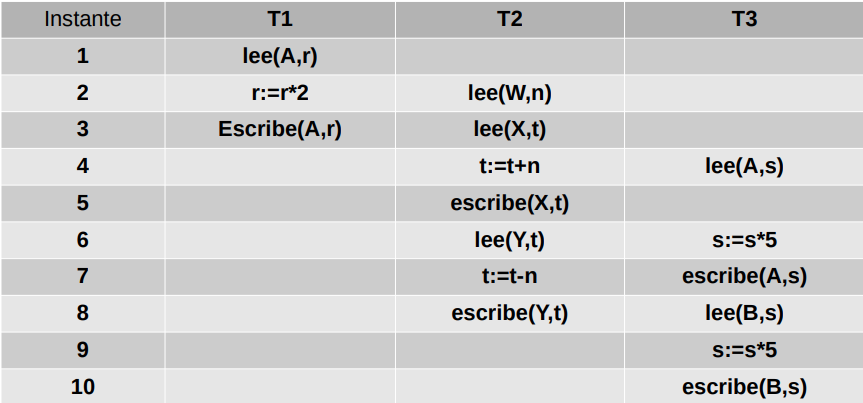
\includegraphics[scale=0.45]{img/20.png}
  \caption{Ejemplo de transacciones}
\end{figure}

\begin{figure}[H]
  \center
  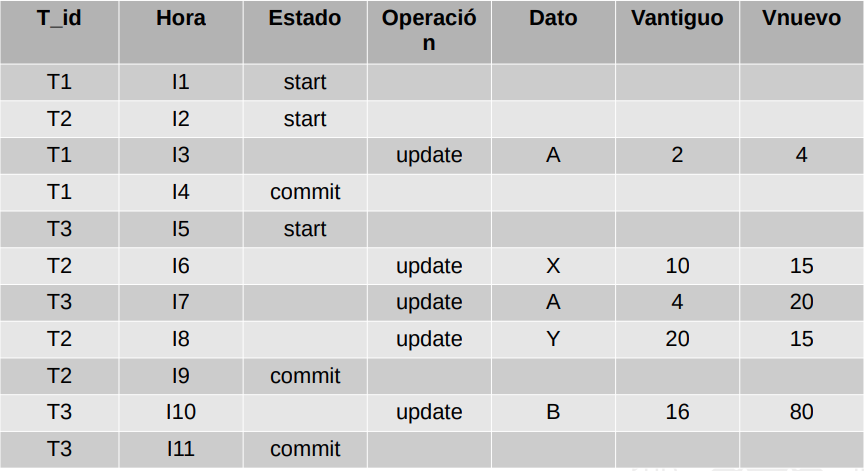
\includegraphics[scale=0.45]{img/21.png}
  \caption{Bitácora asociada a las transacciones anteriores}
\end{figure}

Ojo que las operaciones de lectura como no pueden producir fallos de los que haya que recuperarse, no generan ninguna entrada en la tabla de modificaciones. Las modificaciones a las variables de memoria tampoco generan entradas. Las transacciones tampoco tienen que terminar justo después de la última sentencia, pero en este ejemplo hemos supuesto que sí.

\subsection{Modificación diferida de la BD}

La tabla de modificaciones tiene que escribirse en disco (si la dejáramos en memoria se perderían al irse la luz) frecuentemente (sobre todo, después de un commit). De hecho, hasta que la transacción no está guardada en la tabla y está en el disco, no comienza la ejecución real de la transacción (modificaciones en el buffer y de este al disco). De este modo, la ejecución real se aplaza hasta que la transacción esté parcialmente ejecutada.

Normalmente se escriben cada 3 segundos, cuando se llene el 30\% del espacio de la tabla de modificaciones y cuando se ejecuta un checkpoint (puntos donde forzamos el volcado a discos de los datos).

¿Cómo nos recuperamos tras una caída del sistema? Lo primero que se hace es mirar la última copia de la tabla de modificaciones. Las transacciones que no estén parcialmente ejecutadas no han tenido ejecución real y pueden olvidarse (borrándolas de la tabla): $UNDO(T_i)$. Las transacciones parcialmente ejecutadas pueden no haberse ejecutado realmente y es mejor rehacer la transacción volviendo a escribir los valores nuevos : $REDO(T_i)$.

En resumen, $UNDO(T_i)$ se ejecuta cuando hay un \textit{start} pero no un \textit{commit}. $REDO(T_i)$ se ejecuta cuando hay un \textit{start} y un \textit{commit}.

\subsection{Puntos de verificación (checkpoints)}

Se pueden presentar dos problemas con lo planteando anteriormente:
\begin{itemize}
\item La tabla de modificaciones puede ser enorme.
\item Muchas transacciones ya fueron escritas pero no lo sabemos.
\end{itemize}

Para solucionarlos, se introducen los \textbf{checkpoints}. Un checkpoint es un proceso que consiste en:
\begin{enumerate}
\item Grabar la tabla de modificaciones en disco.
\item Guardar los bloques modificados en los datafiles.
\item Escribir un registro checkpoint en la tabla.
\item Graba la tabla de modificaciones en disco.
\end{enumerate}

El algoritmo que incluye los checkpoints en la tabla de modificaciones hace lo siguiente: recorre la tabla de modificaciones que tiene almacenada, de forma que si encuentra un \textit{start} y un \textit{commit} para una transacción, pero después hay un \textit{checkpoint}, entonces sabemos que la transacción ha sido ejecutada normalmente y se ignora. Si hay un \textit{start} antes del checkpoint y un commit después, entonces esa transacción se rehace. Si hay un start después del último checkpoint y no hay commit después del checkpoint, entonces esa transacción se deshace.

\subsection{Transacciones en Oracle}

Oracle usa el mecanismo de \textbf{redo log buffer} y \textbf{redo log file} para implementar las transacciones. Usa dos buffers para que se pueda seguir escribiendo en uno mientras el otro se transfiere a disco. Una transacción comienza en cualquier operación \textit{DML}, y termina cuando pasa una de las siguientes cosas:
\begin{itemize}
\item se hace una llamadqa a \textit{COMMIT} o \textit{ROLLBACK}.
\item se ejecuta una sentencia \textit{DDL}.
\item El usuario se desconecta.
\item El proceso actual termina de forma anormal.
\end{itemize}

\subsubsection{Sentencia COMMIT}

Graba el redo log buffer en el redo log file, da por finalizada la transacción y libera los recursos empleados o bloqueados por la transacción.

\subsubsection{Sentencia ROLLBACK}

Aborta la transacción en curso, deshace los cambios registrados por la transacción abortada y libera los recursos empleados o bloqueados por la transacción.

\subsubsection{Sentencia SAVEPOINT}

Establece un punto de guardado de los cambios con un identificador único. Permite hacer un ROLLBACK a un estado anterior al mismo pero posterior al comienzo de la transacción.

\begin{lstlisting}[ language=SQL,
                    deletekeywords={IDENTITY},
                    deletekeywords={[2]INT},
                    morekeywords={clustered},
                    framesep=8pt,
                    xleftmargin=40pt,
                    framexleftmargin=40pt,
                    frame=tb,
                    framerule=0pt ]
ROLLBACK TO <savepoint name>;
\end{lstlisting}

\section{Salvado y recuperación de una BD}

La persistencia de los datos puede verse comprometida por un fallo en el almacenamiento masivo, por ello, es necesario realizar copias de seguridad. El estado de la base de datos puede recuperarse a partir de la copia de seguridad y rehaciendo las transacciones posteriores a dicha copia.

\subsection{Copia en frío}

Suelen usar aplicaciones del S.O. Debe ser completa y consistente (datafiles, ficheros de control, de instalación, de configuración, etc.). Debe realizarse con la base de datos apagada. En este tipo de copia los ficheros no se interpretan, se copian directamente del disco. Por ejemplo, los redo logs conviene mantenerlos a parte y replicados porque son muy importantes.

En este caso, una copia sólo podrá ser recuperada por otra instalación \textbf{exacta} a la que generó los datos. El procedimiento es el siguiente:
\begin{enumerate}
\item Detener la instancia.
\item Usar los comandos del S.O. para copiar los ficheros correspondientes al dispositivo de copia de seguridad.
\item Iniciar la instancia.
\end{enumerate}

Es problemático en algunas situaciones ya que los usuarios no pueden acceder al sistema mientras se hace la copia (por ejemplo, en los sistemas de alta disponibilidad). Los 'ficheros correspondientes' que hay que incluir en la copia de seguridad de la BD son:
\begin{itemize}
\item Datafiles
\item Control file
\item Redo log files
\end{itemize}
También se recomiendan incluir los ficheros \textit{init.ora} y \textit{config.ora} y el software de aplicaciones actualizado mediante parches.

Para recuperar la BD a partir de una copia en frío, primero tenemos que reinstlar todo el software necesario, aplicarle los parches y crear una base de datos con la misma configuración que la anterior. Una vez hecho eso, derribamos la BD y reemplazamos todos los ficheros nuevos por las copias. Una vez termine, arrancamos de nuevo la BD, como va a usar los control files de la copia de seguridad, se va a hacer referencia a todas las estructuras de la copia.

\subsection{Copia en caliente}

Es realizada por el SGBD. Guarda total o parcialmente objetos de la BD pero sin su estructura interna. Generalmente se conoce como \textit{volcado}. Se puede volver a crear la base de datos \textit{importando} los ficheros resultantes de esta operación.

Permite hacer copia de seguridad con la base de datos en uso por parte de los usuarios. El sistema transfiere las actualizaciones de datos de cualquier transacción terminada (en la tabla de modificaciones). Las nuevas transacciones y transacciones en curso se almacenan en la tabla de modificaciones pero no se transfieren bloques de datos a disco. esto requiere muchos ficheros \textbf{redo log file} numerados de forma consecutiva.

Cuando la copia termine de hacerse, las transacciones se rehacen sobre los datafiles para almacenar los cambios. Este modo se llama \textbf{archivelog mode} y debe estar habilitado.

El principal problema es que no se puede hacer por ejemplo copia de seguridad del catálogo, ya que siempre está en uso. Además enlentece el sistema, por lo tanto no se recomienda hacer cuando la BD está siendo muy usada.

Procedimiento para realizar la copia:
\begin{lstlisting}[ language=SQL,
                    deletekeywords={IDENTITY},
                    deletekeywords={[2]INT},
                    morekeywords={clustered},
                    framesep=8pt,
                    xleftmargin=40pt,
                    framexleftmargin=40pt,
                    frame=tb,
                    framerule=0pt ]
ALTER TABLESPACE <nombre> BEGIN BACKUP;
HOST xcopy <ruta>\<nombre>*.dbf <destino>;
ALTER TABLESPACE <nombre> END BACKUP;
\end{lstlisting}
La vista $\$backup$ nos da información sobre el estado de los backups.

Cuando un tablespace o uno de sus datafiles produce un fallo, se pueden reemplazar por una copia anterior. El proceso sustituye los datafiles y aplica todos los cambios posteriores a la copia a partir de los históricos de ejecución:
\begin{lstlisting}[ language=SQL,
                    deletekeywords={IDENTITY},
                    deletekeywords={[2]INT},
                    morekeywords={clustered, recover, tablespace},
                    framesep=8pt,
                    xleftmargin=40pt,
                    framexleftmargin=40pt,
                    frame=tb,
                    framerule=0pt ]
# se recupera un tablespace entero
RECOVER TABLESPACE <nombre>;
# solo se recupera el fichero que ha fallado
RECOVER DATAFILE <ruta>;
# base de datos entera
RECOVER DATABASE;
\end{lstlisting}

\subsection{Copia lógica}

Consulta la BD y el catálogo para crear un \textit{fichero binario} con los objetos seleccionados, de extensión .dmp. Puede hacerse de la base de datos completa, un usuario concreto (o varios) o una tabla concreta (o varias). Permite almacenar información de catálogo correspondiente al objeto u objetos salvados (privilegios, índices, restricciones).

Las exportaciones de la BD se llaman \textbf{completas} y las de tablas modificadas se llaman \textbf{incrementales}.

Para recuperar una copia, Oracle permite leer un fichero .dmp recuperando su contenido sobre una base de datos y especificando el usuario que creará los objetos recuperados.

\subsection{Criterios para elegir uno u otro}

\begin{itemize}
\item Se elige siempre un método primario, y otro en caso de que este falle.
\item La copia en frío sólo se usa cuando fallan los demás.
\item En bases de datos orientadas a las transacciones, es mejor la copia en caliente.
\item Si se usa exportación, tendremos que conformarnos con el estado de la BD cuando se exportó.
\item Cualquier procedimiento debería incluir una exportación y una copia física.
\end{itemize}